\documentclass[pdflatex,sn-nature]{sn-jnl}

\usepackage{graphicx}
\usepackage{multirow}
\usepackage{amsmath,amssymb,amsfonts}
\usepackage{booktabs}
\usepackage{xcolor}
\usepackage{float}
\usepackage{url}

\newcommand{\placeholder}[1]{\textcolor{red}{[PLACEHOLDER: #1]}}
\newcommand{\figref}[1]{Fig.~\ref{#1}}

\raggedbottom

\begin{document}

\title[Controllability is not extrapolation]{Conditioning improves in-support controllability but does not produce true property extrapolation in polymer generative models}

\author*[1]{\fnm{Yi} \sur{Cao}}\email{\placeholder{corresponding-author-email}}
\affil*[1]{\orgname{Toyota Research Institute}, \orgaddress{\city{Los Altos}, \state{California}, \country{USA}}}
\author[2]{\fnm{\placeholder{Coauthor}} \sur{\placeholder{Surname}}}
\affil[2]{\orgname{\placeholder{Affiliation}}}

\abstract{Conditional generative models are increasingly used to propose molecules with desired properties, but a central distinction is often left implicit: steering samples within the training support is not the same as generating candidates beyond the observed frontier. Here we establish a staged, support-aware benchmark for polymer electrolyte generation and apply it to a character-level autoregressive PolyGen model trained from scratch on a single high-throughput molecular-dynamics source. Continuous conditioning improves target adherence over a binary baseline at in-support quantiles and remains usable near the upper boundary, while incurring a modest validity and novelty trade-off. However, when the target is moved to the 90th and 100th percentiles or beyond the maximum training conductivity, neither continuous nor binary conditioning produces a surrogate-supported frontier crossing across five matched seeds. An independent six-property conditioning experiment reaches the same negative result: no arm produces a strict joint hit or an all-property frontier crossing. These results define a practical evaluation boundary for conditional molecular generation and motivate future gains through broader labelled data, richer molecular representations and closed-loop validation rather than finer conditioning alone.}

\keywords{polymer electrolytes, molecular generation, conditional generation, extrapolation, controllability, active learning}

\section*{Introduction}
The design of polymer electrolytes requires navigating a coupled chemical and transport landscape in which the most useful candidates may lie close to, or beyond, the best observed conductivity. Generative models promise to reduce this search burden by proposing polymer repeat units conditioned on a target property. Yet a model can appear controllable while merely reweighting structures already represented in its training distribution. A convincing claim of extrapolation therefore requires an explicit boundary, an evaluation region outside that boundary and a verifier that is not the generator objective itself.

We revisit this distinction in a reproducible PolyGen benchmark. The study is deliberately narrow: a character-level autoregressive generator is trained from scratch on a single high-throughput molecular-dynamics (HTP-MD) source, and generated structures are evaluated with a frozen random-forest (RF) surrogate. This design does not establish experimental discovery. Instead, it isolates what conditioning can and cannot do under a fixed data and representation regime.

Our contribution is a four-stage evaluation ladder: interpolation within the training support, upper-tail control near the observed boundary, true numerical extrapolation beyond the training maximum, and structural out-of-distribution evaluation. The first three stages are completed here; the last remains blocked by missing scaffold and family annotations. The central result is a clean separation between controllability and extrapolation. Continuous conditioning improves in-support target adherence, but both continuous and binary conditioning fail the strict frontier-crossing test at every extrapolation query. A six-property joint-conditioning experiment, motivated by recent multi-property molecular generation, reproduces the same limitation.

This negative result is scientifically useful. It identifies the current bottleneck as a limitation of data coverage and representation, rather than a failure to tune the conditioning label finely enough. It also gives a concrete standard for future work: claims of property extrapolation must report support, validity, uncertainty, and an independently defined frontier-crossing criterion.


\section*{Results}
\subsection*{In-support controllability improves with continuous conditioning}

We first evaluated targets at the training-distribution quantiles Q50, Q65 and Q80 using five matched seeds (17, 42, 202, 303 and 907), 100 generated candidates per arm, target and seed, and identical decoding settings. The continuous arm improved mean strict-hit rate from 0.159 to 0.178 and reduced target MAE from 0.694 to 0.633 across the three target levels, while validity decreased from 0.522 to 0.455 and novelty from 0.503 to 0.431. These are RF-screening metrics, not MD- or experimentally measured conductivity.

\begin{figure}[H]
\centering
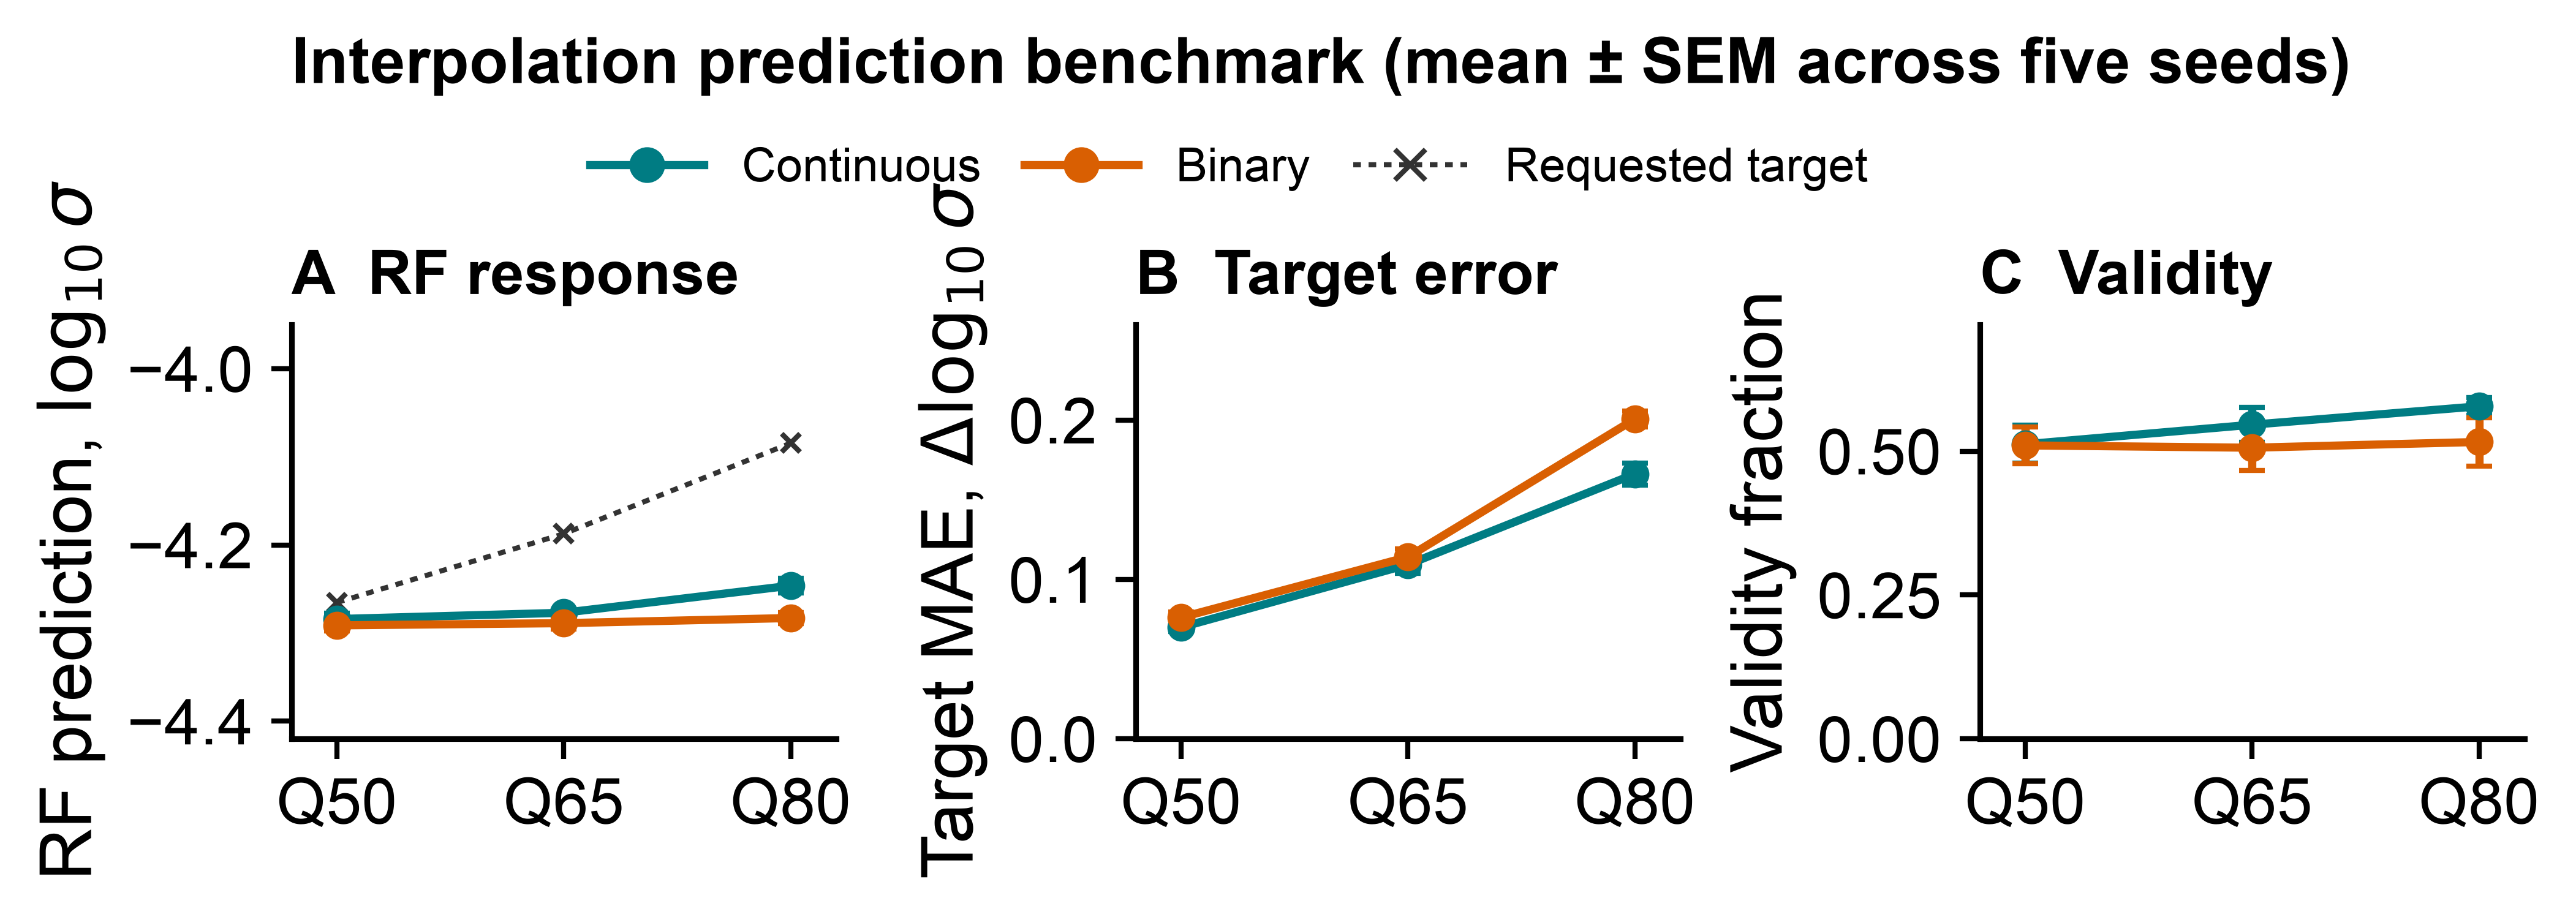
\includegraphics[width=0.98\linewidth]{figures/Figure_1_interpolation_response.png}
\caption{In-support response. Continuous conditioning improves target adherence across the interpolation targets relative to the binary baseline, but performance remains a trade-off between target error and the yield of valid and novel structures.}
\label{fig:interpolation-response}
\end{figure}

The paired design supports a restrained interpretation. The mean strict-hit improvement was 0.0193, positive for all five seeds, but the small number of seeds and the support-limited nature of the task make this exploratory rather than confirmatory evidence. Candidate-wise target ordering was more monotonic for continuous conditioning (0.991 mean correlation) than for binary conditioning (0.873), consistent with a more informative conditioning signal. It does not imply that the model learned a globally valid conductivity map.

\begin{figure}[H]
\centering
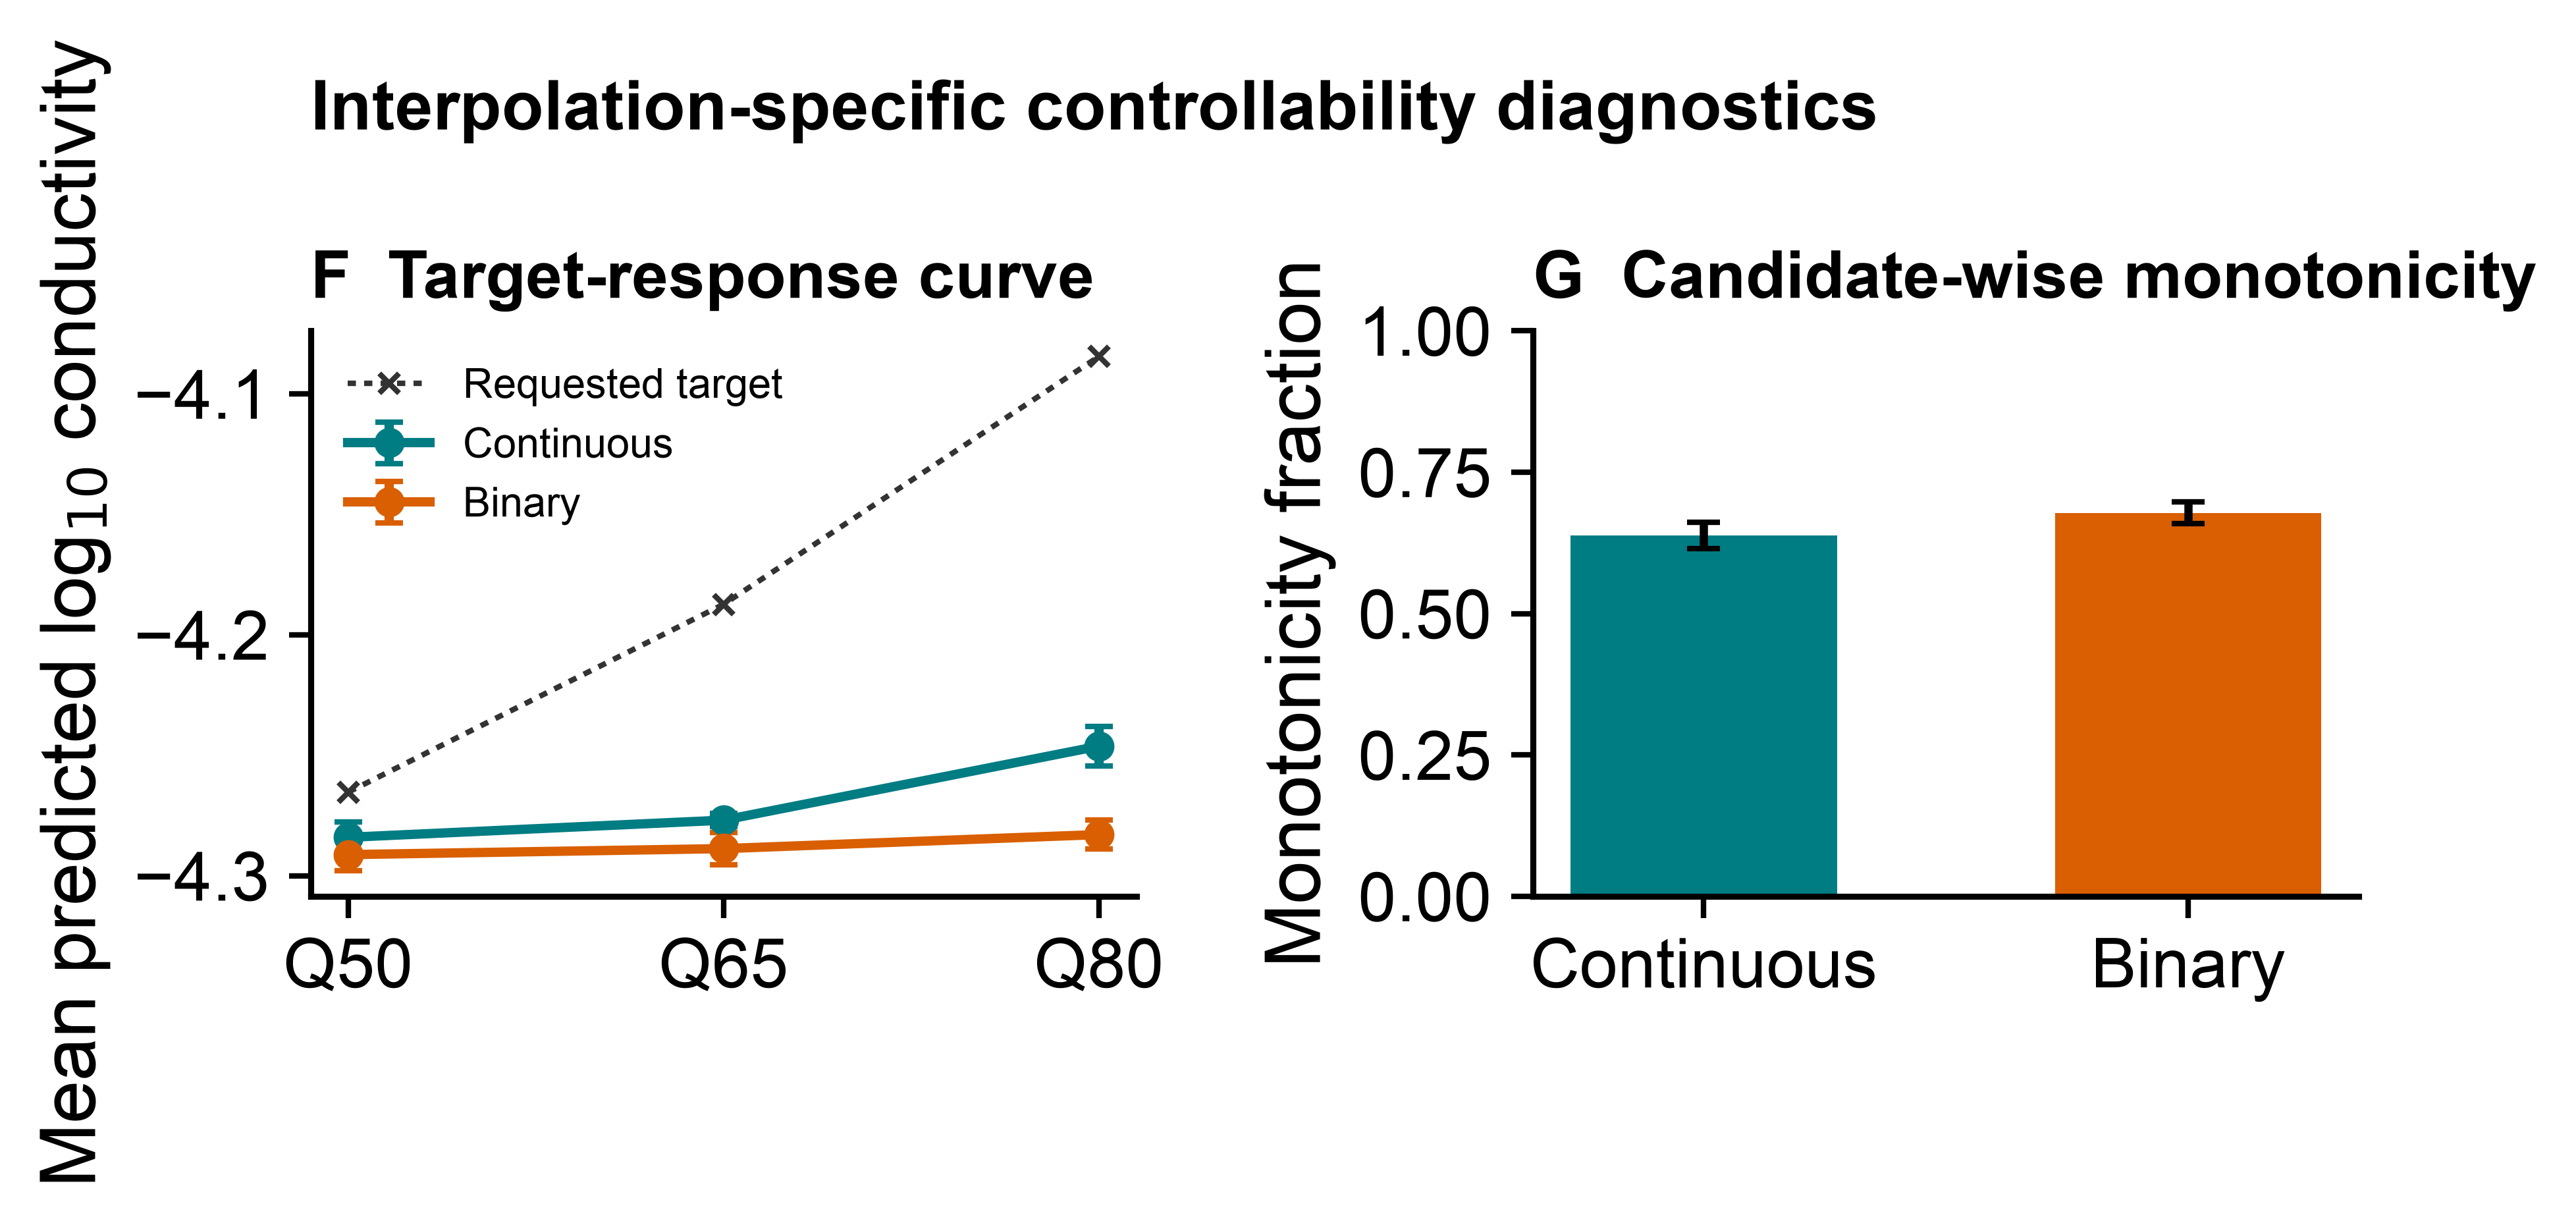
\includegraphics[width=0.98\linewidth]{figures/Figure_3_interpolation_controllability.png}
\caption{Controllability diagnostics across target quantiles. The continuous arm provides a smoother target response within the observed support, while quality and support filters remain essential for interpreting generated candidates.}
\label{fig:interpolation-controllability}
\end{figure}

\subsection*{Control persists near the boundary, but the boundary is not crossed}

We next moved the target from the actual training maximum (Q80 boundary) through Q85, Q90 and Q95. Continuous conditioning remained operational in every matched cell, with validity between 0.56 and 0.584 and strict-hit rates between 0.522 and 0.570. Binary conditioning remained usable at the boundary and Q85, but its fixed threshold became single-class after Q80 truncation; all five Q90 and Q95 cells were therefore unsupported rather than silently treated as zero-quality successes.

\begin{figure}[H]
\centering
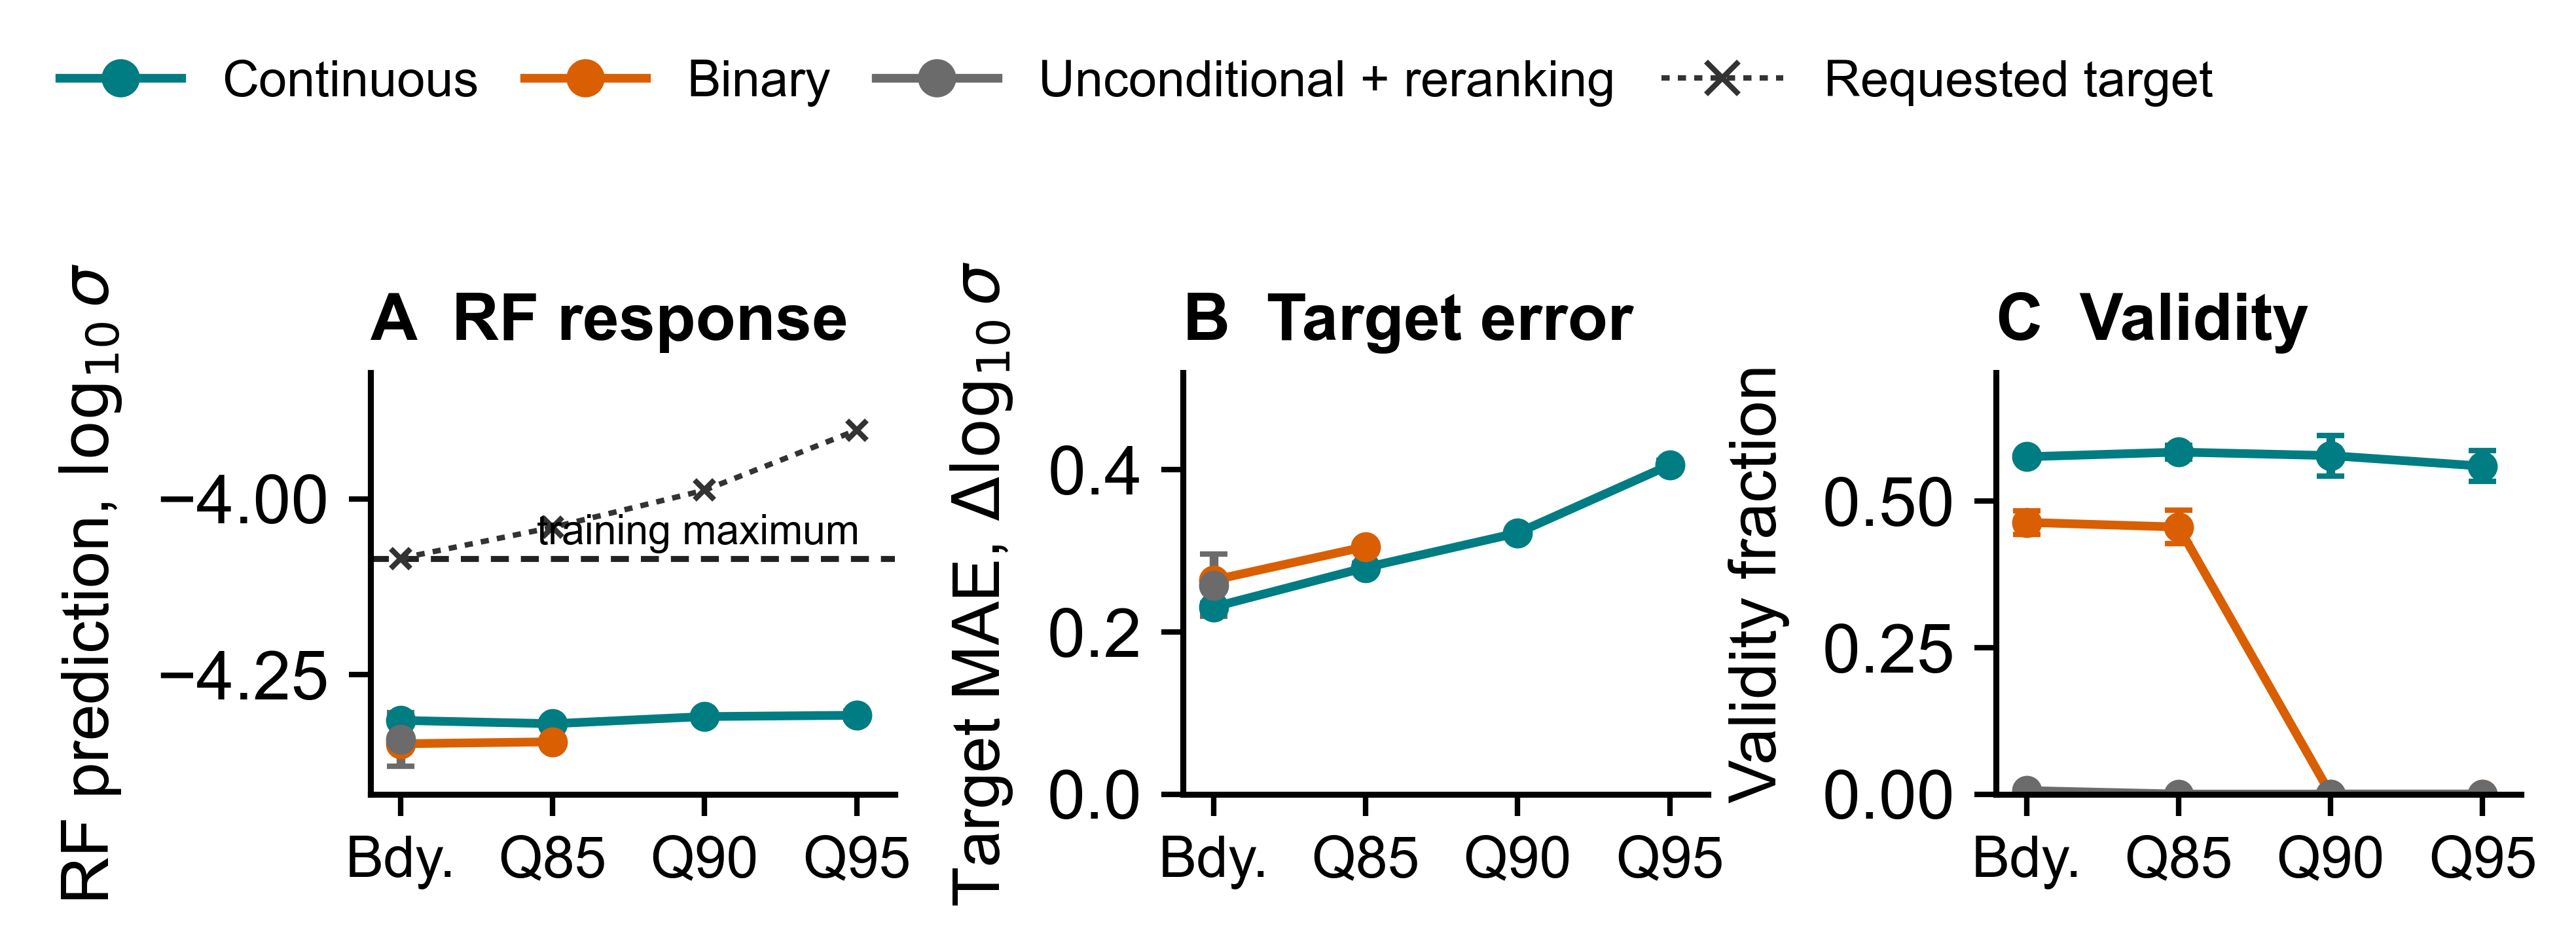
\includegraphics[width=0.98\linewidth]{figures/Figure_1_upper_tail_response.png}
\caption{Upper-tail response. Continuous conditioning degrades gradually as the target approaches the training frontier; binary conditioning becomes structurally unsupported when its fixed threshold cannot encode the requested region.}
\label{fig:upper-tail-response}
\end{figure}

The RF predictions also remained below the requested targets in this regime: the upper-tail predicted-hit rate was 0.0 for every arm and query in the locked audit. Thus the upper-tail experiment measures boundary approach and support degradation, not successful extrapolation. This distinction motivates the next benchmark.

\subsection*{True extrapolation fails under both conditioning schemes}

The frozen training boundary was $-4.084499111$ in $\log_{10}(\mathrm{S\,cm^{-1}})$, with 4,819 rows at or below full-source Q80. We evaluated Q90, Q100, and targets at the training maximum plus 0.25 and 0.50 log units. The benchmark used continuous conditioning, the fixed-threshold binary negative control and an unconditional reranking arm, with five matched seeds and the same 1,000-step, temperature-1.0, top-k-40 protocol.

The decisive metric was \emph{frontier-crossing predicted hit rate}: the fraction of candidates that passed validity, novelty, support and uncertainty gates and whose independent RF prediction crossed the frozen training boundary in the requested direction. This rate was 0.0 for continuous conditioning at all four queries and 0.0 for binary conditioning at all four queries. For continuous conditioning, validity fell from 0.564 at Q90 to 0.280 at Q100; at train-max+0.50, validity was 0.390 and target MAE was 0.718, but the mean RF prediction remained near $-4.30$, below the training frontier.

\begin{figure}[H]
\centering
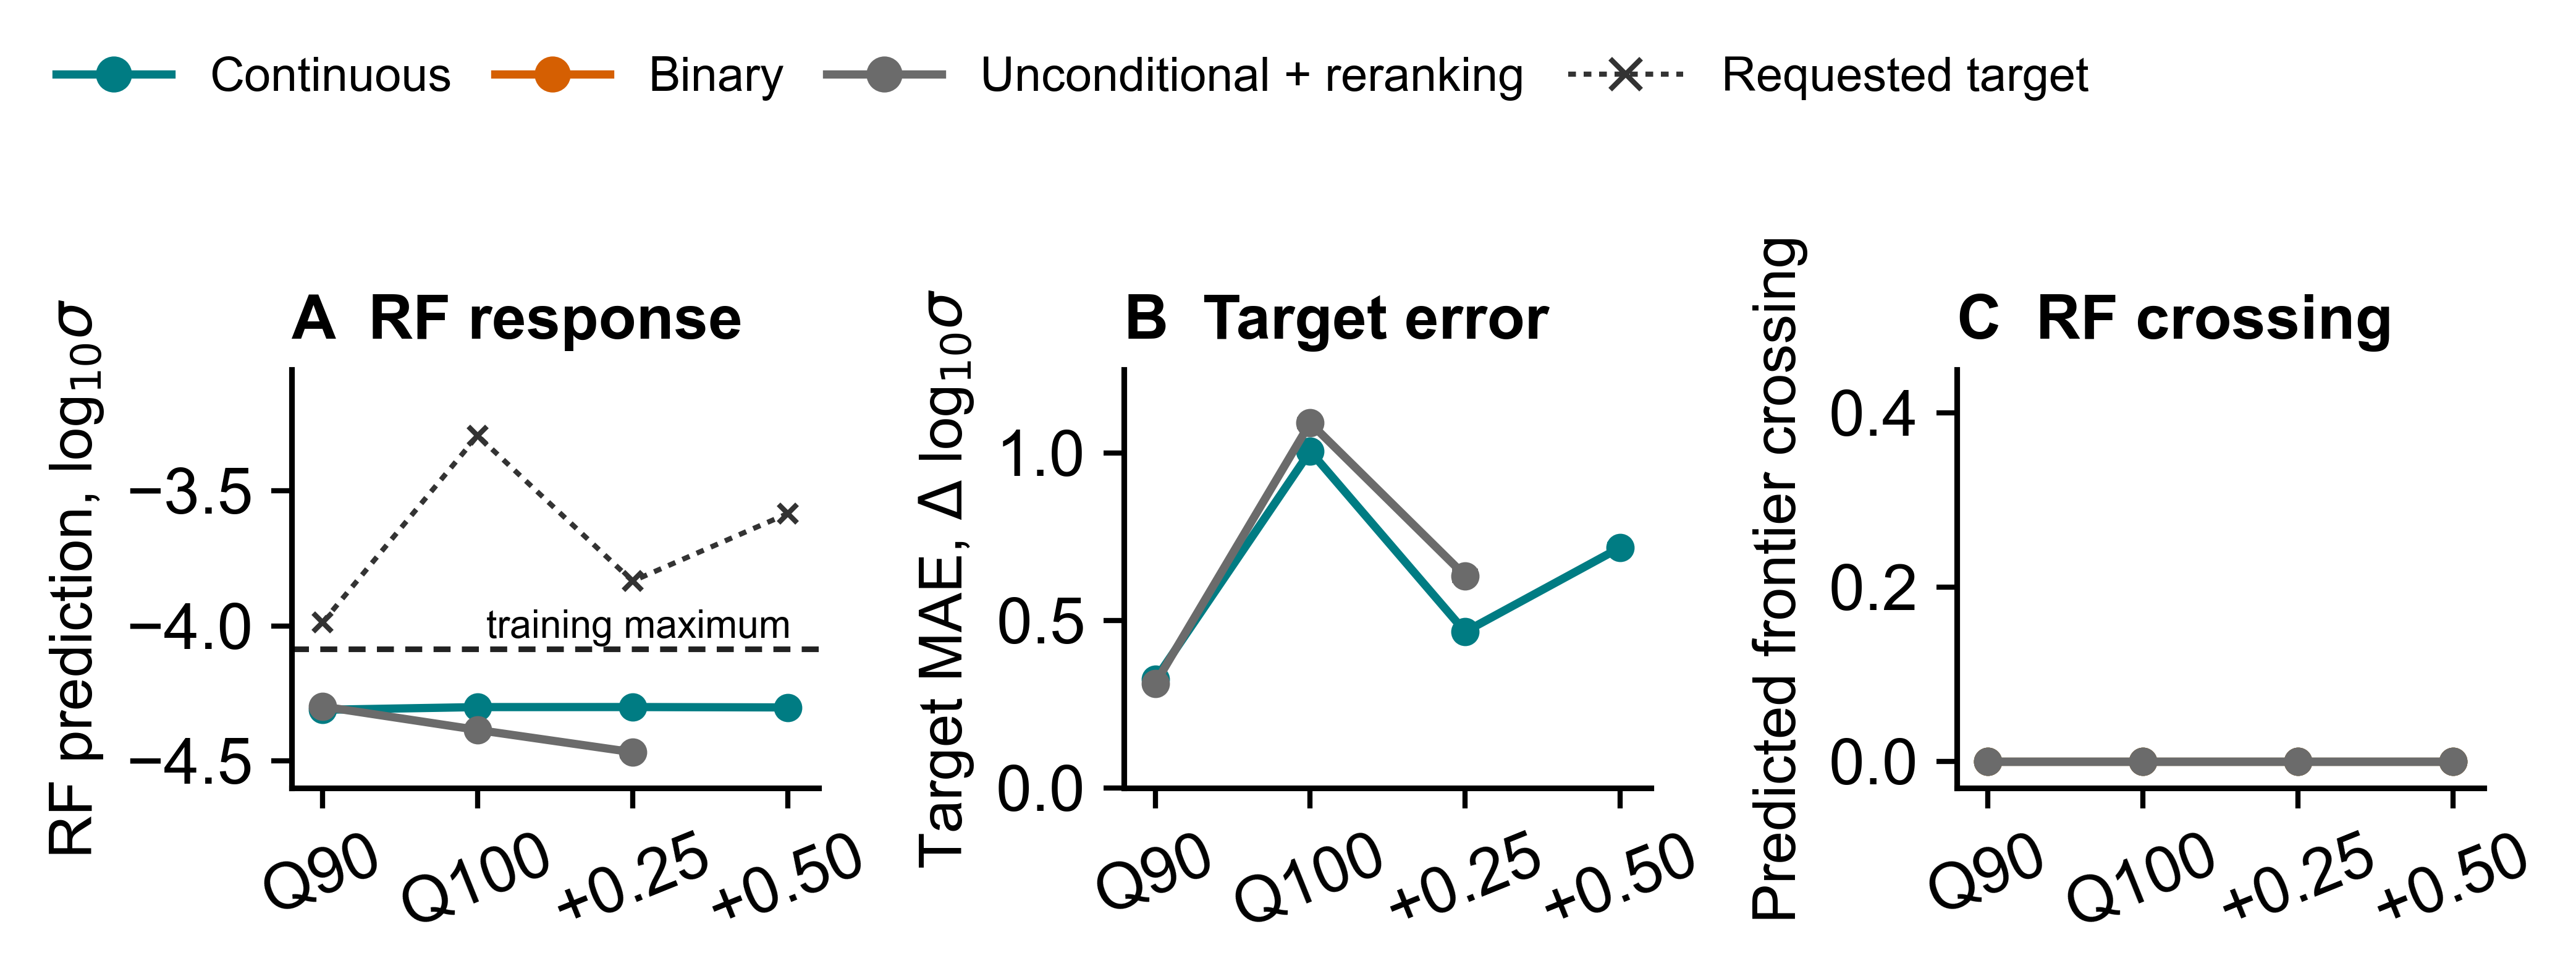
\includegraphics[width=0.98\linewidth]{figures/Figure_1_extrapolation_response.png}
\caption{True extrapolation response. Requested targets move beyond the frozen training support, but RF-predicted candidates do not cross the training frontier for either continuous or binary conditioning.}
\label{fig:extrapolation-response}
\end{figure}

\begin{figure}[H]
\centering
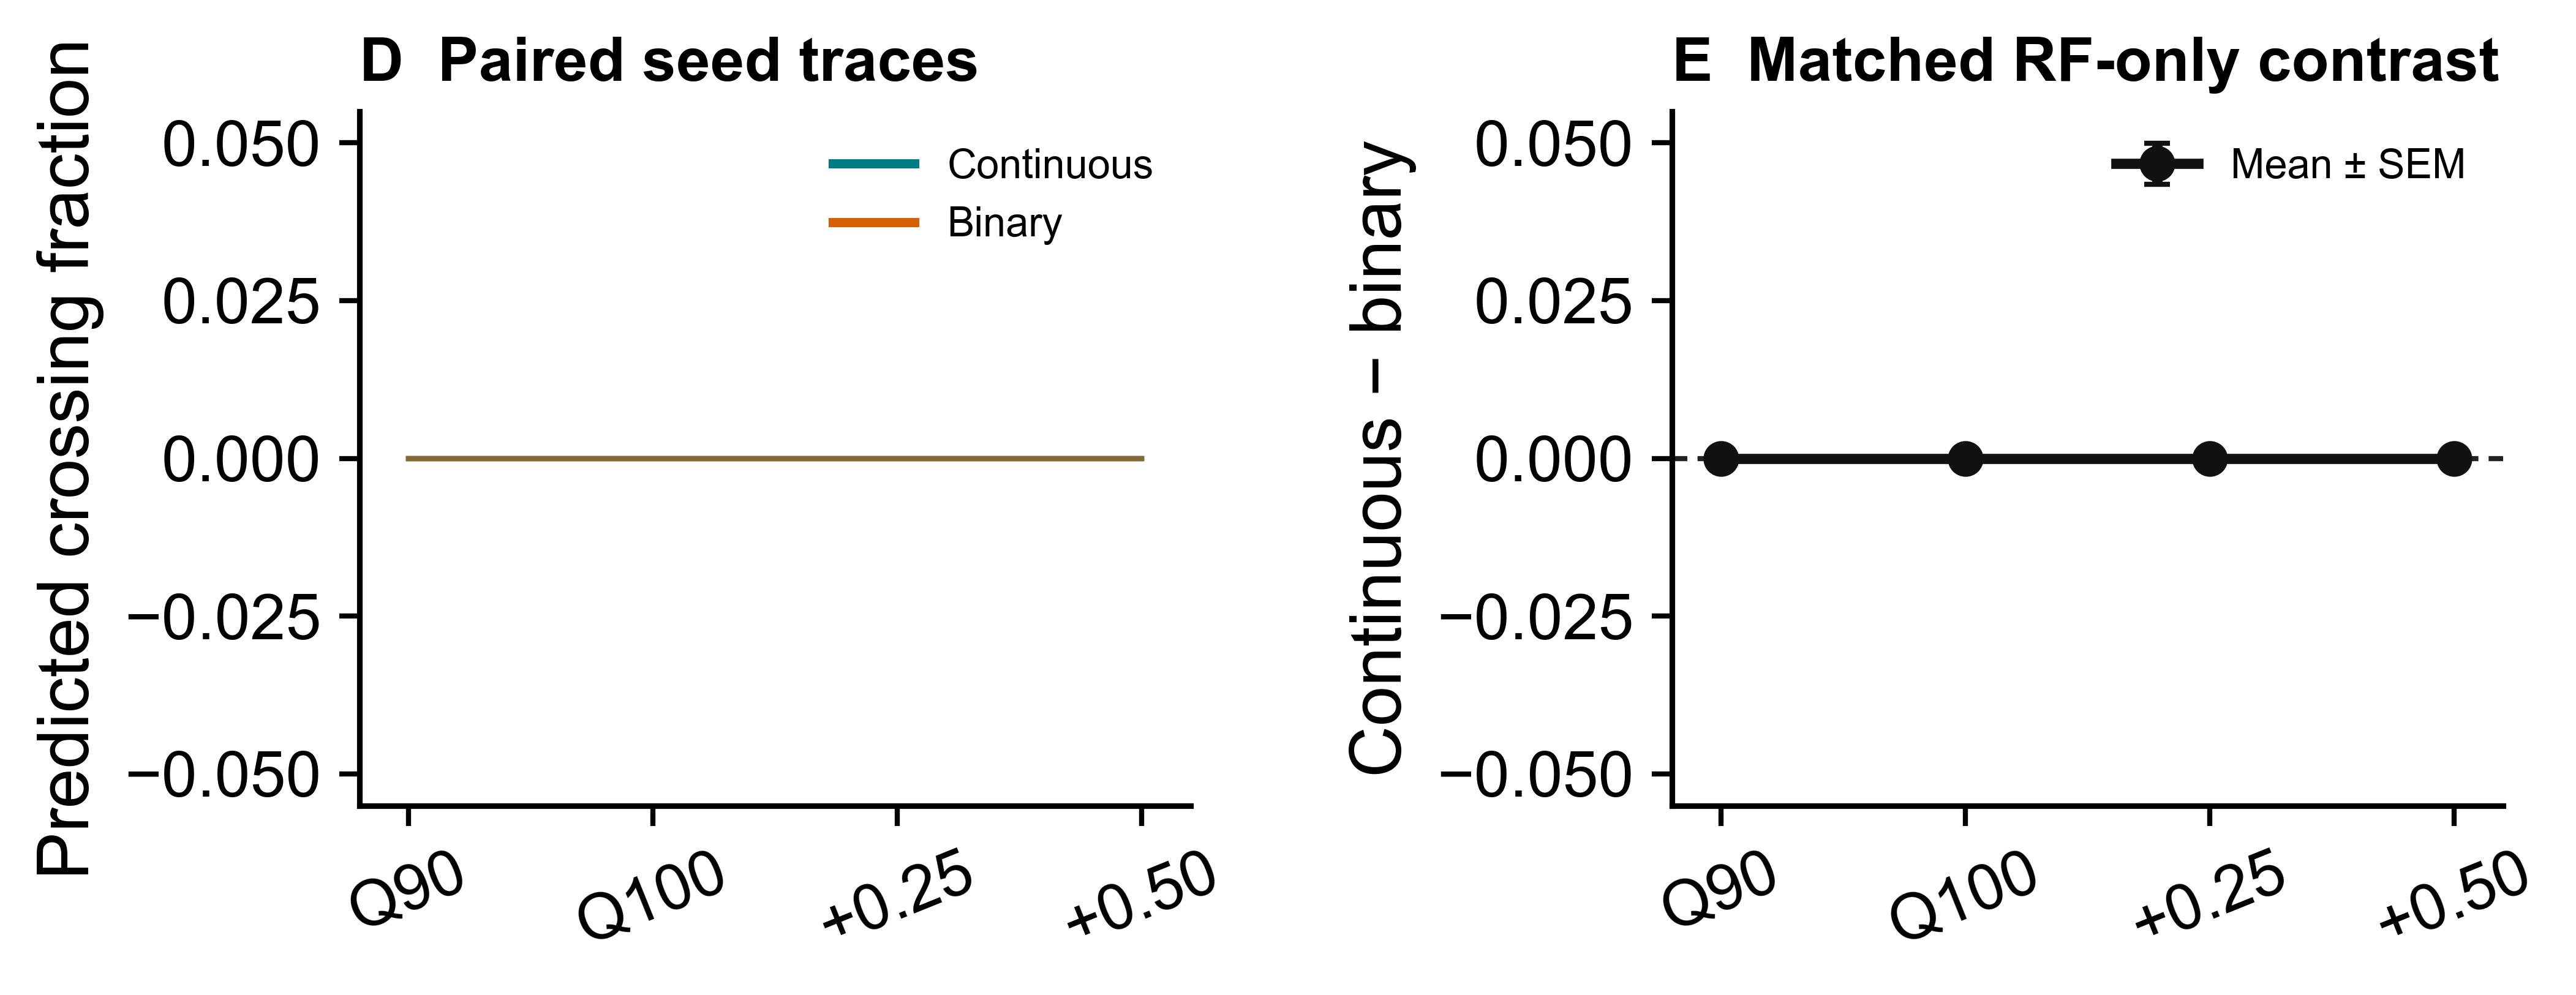
\includegraphics[width=0.98\linewidth]{figures/Figure_2_extrapolation_paired_contrast.png}
\caption{Paired extrapolation contrast across five seeds. Differences between conditioning arms do not change the zero frontier-crossing conclusion.}
\label{fig:extrapolation-contrast}
\end{figure}

This result is not evidence that the generator never produces high-scoring structures under any verifier. It is a narrower and stronger statement: under the frozen HTP-MD data source, representation and protocol, no arm generated a candidate that simultaneously satisfied the pre-registered validity/support/uncertainty gates and crossed the independently audited RF frontier. MD was not run by contract, so no physical or experimental extrapolation claim is made.

\subsection*{Six-property conditioning does not remove the frontier bottleneck}

To test whether the limitation was specific to a single scalar label, we evaluated a parallel six-property conditioning benchmark on the Q80 intersection (2,494 of 6,024 rows). The joint target vector comprised conductivity, lithium diffusivity, TFSI diffusivity, polymer diffusivity, transference number and molality. The benchmark compared multi-property conditioning with scalar-conductivity conditioning, binary conditioning and unconditional reranking.

Across Q90, Q100, train-max+0.25 and train-max+0.50, no arm produced a strict joint hit or an all-six-property frontier crossing. The result is consistent with the scalar experiment: increasing the number of conditioning coordinates improves the specification of the target, but does not create training support where none exists.

\begin{figure}[H]
\centering
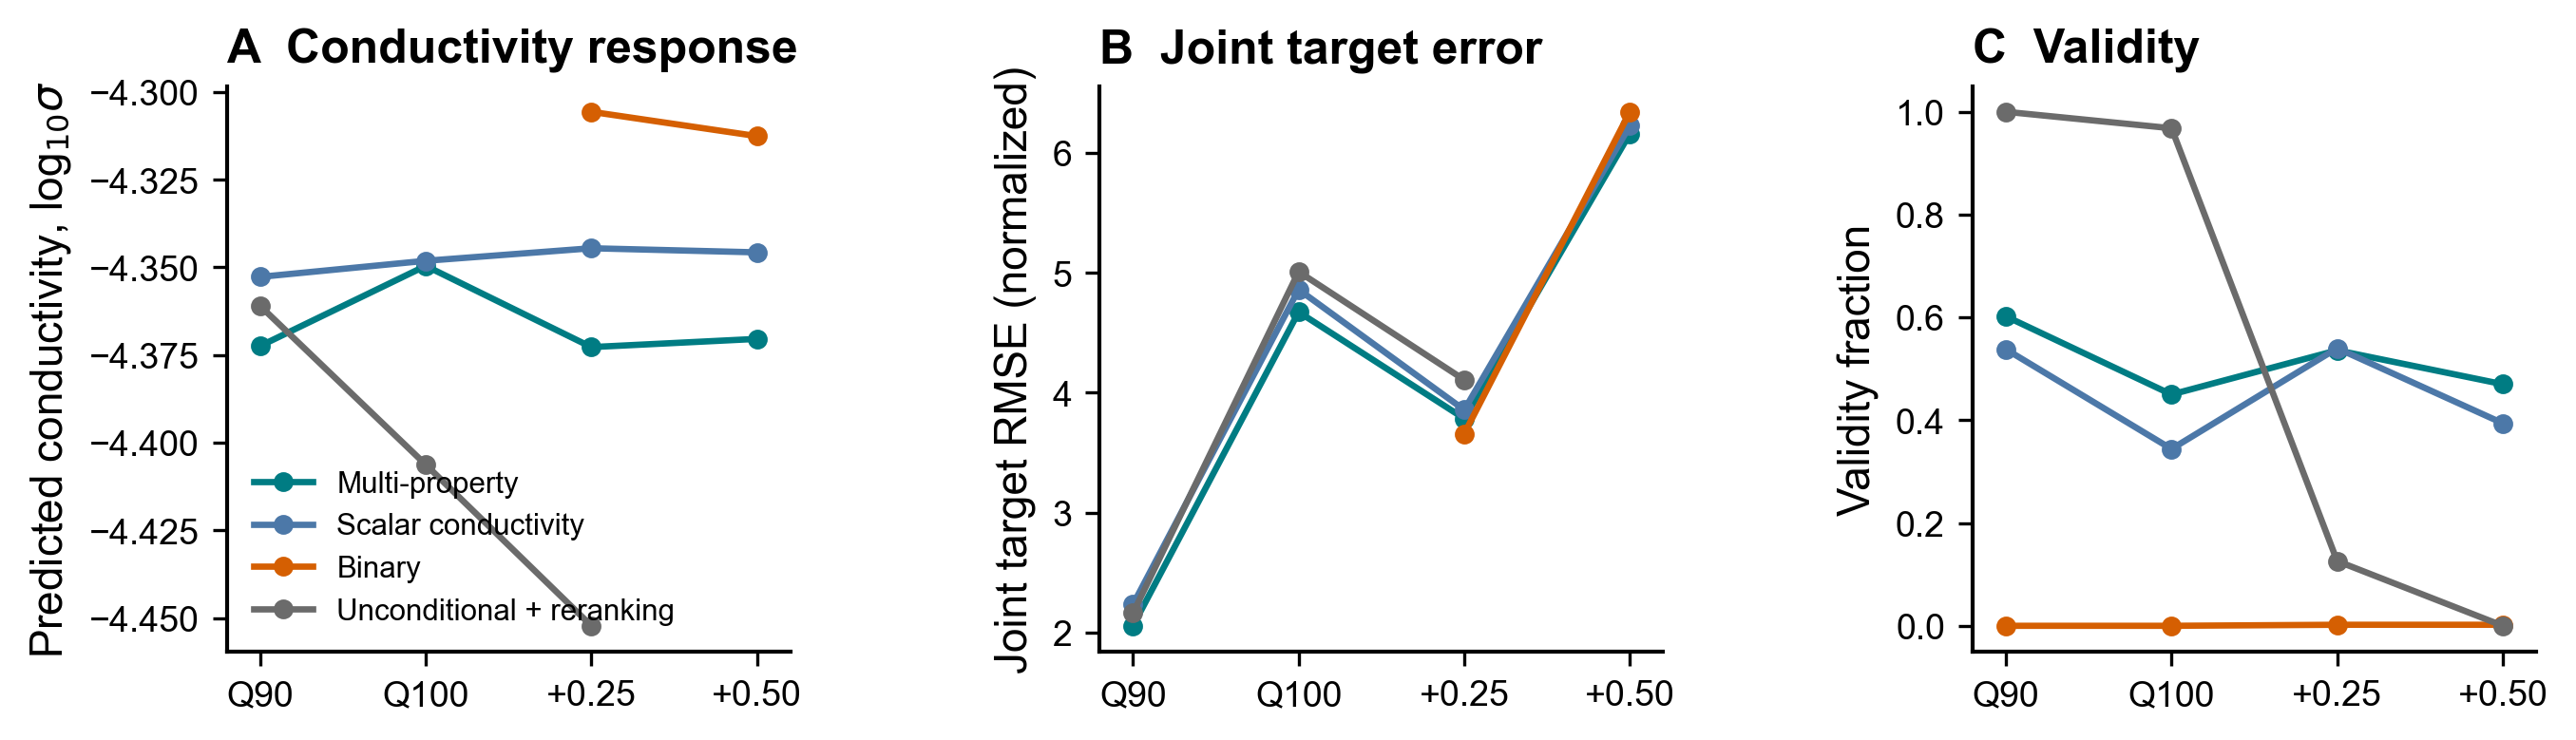
\includegraphics[width=0.98\linewidth]{figures/Figure_1_multi_property_response.png}
\caption{Joint-property extrapolation response. Multi-property conditioning produces no strict joint hit or all-property frontier crossing in the extrapolation regions.}
\label{fig:multi-property-response}
\end{figure}

This parallel result is particularly important for interpreting multi-property generation papers. A richer conditioning vector can enable in-support re-ranking or target trade-offs without establishing out-of-support generalization. Here, the all-property frontier criterion makes that distinction explicit.


\section*{Methods}
\subsection*{Generator and conditioning arms}

The generator is a character-level autoregressive GPT-style model trained from scratch on the released HTP-MD polymer dataset. The continuous arm receives a numerical conductivity condition, whereas the binary arm receives the original fixed-threshold label. All comparisons use matched seeds, decoding budgets and temperature/top-$k$ settings. The unconditional reranking arm is treated as a diagnostic control and not as a fully independent unconditional generator where a released checkpoint is unavailable.

\subsection*{Data splits and evaluation ladder}

The training boundary is frozen before generation. Interpolation targets are Q50, Q65 and Q80. The upper-tail targets are the actual training boundary, Q85, Q90 and Q95. True extrapolation targets are Q90, Q100, train-max+0.25 and train-max+0.50; the locked Q80--Q100 tail is reserved for verifier auditing. Each cell contains 100 generated candidates per seed and arm unless a documented structural or threshold failure prevents generation.

\subsection*{Validity, support and frontier crossing}

Candidate validity is determined by the released structural parser and polymer end-count checks. Novelty is assessed against the generator training set. The RF verifier supplies predicted conductivity and uncertainty. A strict hit requires a valid, novel and support-eligible candidate whose absolute target error is within the frozen tolerance and whose uncertainty passes the audit threshold. A frontier crossing additionally requires the RF prediction to exceed the frozen training maximum. Empty or single-class cells are recorded as unsupported failures, not imputed as successful or comparable samples.

\subsection*{Multi-property audit}

The joint benchmark uses the intersection of rows with all six measured properties and applies the same validity, novelty, support, uncertainty and joint-error gates. A strict joint hit requires all six target errors to satisfy the frozen normalized threshold; an all-property frontier crossing requires the corresponding property-level frontier conditions to be met simultaneously.

\subsection*{Statistical reporting}

We report five-seed means and standard errors for descriptive comparison. Paired seed contrasts are used because the same seeds and decoding settings are shared between arms. Given the small number of independent seeds and the RF-only verifier boundary, results are presented as benchmark evidence rather than population-level estimates of experimental performance.


\section*{Discussion}
\subsection*{Conditioning is a controllability mechanism, not an extrapolation mechanism}

The experiments support a simple but consequential conclusion. Continuous conditioning is useful: it improves target adherence and preserves usable generation closer to the observed boundary than the fixed-threshold binary baseline. But the same mechanism does not create reliable candidates beyond the boundary. The zero frontier-crossing result at Q90, Q100 and both train-max offsets is unchanged by moving from one property to six.

This observation also clarifies how to compare the present benchmark with fragment-based or multi-property molecular generators such as MolMiner. In-support enrichment, target ordering and Pareto reweighting are valuable capabilities, but none is by itself evidence of numerical OOD extrapolation. A fair comparison must freeze the training support, define the frontier before generation and audit candidate predictions against that boundary.

The practical implication is that the next gain is unlikely to come from conditioning design alone. The most promising directions are: (i) adding genuinely labelled conductivity data from harmonized experimental sources, rather than using an unlabelled DFT database as if it supplied conductivity; (ii) testing fragment-based or otherwise richer representations; and (iii) coupling generation to active-learning or MD validation so that new frontier regions become labelled and feed back into the model.

\placeholder{Add literature citations and a quantitative comparison to the final MolMiner manuscript once the bibliography and exact comparator protocol are frozen.}


\section*{Limitations and outlook}
The present study has four deliberate limitations. First, the verifier is a released RF model; no extrapolation candidate has been confirmed by molecular dynamics or experiment. Second, the data source is a single HTP-MD protocol, so the conclusions are conditional on its chemistry and simulation support. Third, structural-OOD evaluation is blocked because scaffold/family annotations and matched continuous/binary checkpoints are not yet available. Fourth, the six-property benchmark is a prediction-phase audit and should not be interpreted as a validated multi-property physical model.

The next study should therefore begin with provenance-preserving expansion of the labelled conductivity corpus, followed by a representation ablation and a closed-loop acquisition experiment. A larger unlabelled database such as OPoly26 may be useful for geometry or force-field pretraining, but it cannot directly expand the conductivity label space. Active learning should be evaluated after MD calibration and with a pre-registered acquisition criterion.\

\placeholder{Insert final MD validation results, external-data calibration, structural-OOD split and active-learning results when available.}


\section*{Data and code availability}
All numerical claims in this draft are derived from the local PolyGen-reproduction evidence package. The canonical analysis repository is \url{https://github.com/yicao-tri/PolyGen-reproduction}; the exact commit, data hashes and release DOI are \placeholder{to be filled after the evidence package is committed}. Generated candidates, frozen manifests, aggregate metrics and publication figures are retained under the corresponding \texttt{results/} subdirectories. No candidate in this manuscript is presented as MD- or experimentally validated.

\placeholder{Add author contributions, competing interests, ethics statement if required, funding, and final data/code DOI.}


\bibliography{sn-bibliography}

\end{document}
